\documentclass[12pt,a4paper]{article}
\usepackage[utf8]{inputenc}
\usepackage[T1]{fontenc}
\usepackage{titling}
\usepackage{amsfonts}
\usepackage{amssymb}
\usepackage{amsmath}
\usepackage{tcolorbox}
\usepackage{mdframed}
\usepackage{graphicx}
\usepackage{wrapfig}
% \usepackage{libertine}
\usepackage{tikzpagenodes}
\usepackage{float}
\usepackage{amsfonts}
\usepackage[top=1in, bottom=1.5in, left=1in, right=1in]{geometry}
\renewcommand{\contentsname}{Sadržaj}

\setlength{\droptitle}{-8em}


\title{\vspace{-2.3cm}\Large \textsc{univerzitet u novom sadu
\\prirodno-matematički fakultet
\\departman za
\\matematiku i informatiku}
\vspace{5em} 
\\ \textbf{Remzijevi brojevi}
\\ \large - seminarski rad -
\vspace{1em} }


\graphicspath{ {GeogebraSlike/} }

\begin{document}

	\begin{figure}[]
	\centering
	\advance\leftskip-14cm
	
\includegraphics[scale=0.3]{logo1.png}
	\end{figure}
	

	\begin{figure}[]
	\vspace{-3.4cm}
	\centering
	\advance\leftskip14cm
	
\includegraphics[scale=0.3]{logo2.png}
	\end{figure}

	\author{
  	Renea Mošo\\
  	\texttt{}
  	\and
  	Nikola Obradović\\
  	\texttt{}
  	\and
  	Nikola Pešić
	}	
	\date{}
	
	
	\maketitle
	
	\thispagestyle{empty}
	
	\newpage
	
	
	\tableofcontents
	\newpage
	
	\section{Uvod u Remzijevu teoriju}
	
	\noindent Naziv je dat u čast britanskog matematičara, Frank Plumpton Ramsey-a, koji je objavio članak
	1928. sa dokazom koji je danas poznat kao Remzijeva teorija. Opšte shvatanje ove teoreme često glasi:
	''U svakom neredu postoji red.'', ali shvatanje koje je prikladnije ovom radu je ideja da svaka
	struktura sadrži uređenu podstrukturu. Međutim, da bismo shvatili Remzijevu teoriju, moramo uvesti
	određene matematičke pojmove.

	\subsection{Dirihlet-ov princip}
	\vspace{0.5em}
	
	Počnimo najpre od jednog opšte poznatog problema.	
	\vspace{0.5em}
	\\
	{\noindent\fontsize{12pt}{12pt}\textbf{Primer}}
	\vspace{0.5em}
 	
	\noindent Ako se $n + 1$ zečeva smesti u n kaveza, onda će se bar dva zeca naći u istom kavezu.
	\vspace{1.5em}

	{\noindent\fontsize{12pt}{12pt}\textbf{Dokaz}}
	\vspace{0.5em}	

	\noindent Pretpostavimo da svaka kutija sadrži najviše jednog zeca. Tada je ukupan broj zečeva
	najviše n, što je u suprotnosti sa pretpostavkom da ima n + 1 zečeva. 
	\vspace{1.5em}	

	{\noindent\fontsize{12pt}{12pt}\textbf{Teorema 1.1}}
	\vspace{0.5em}

	\noindent Ako su $A$ i $B$ konačni skupovi i |A| > |B|, onda ne postoji injektivno preslikavanje skupa A u
	skup B.
	\vspace{1.5em}

	{\noindent\fontsize{12pt}{12pt}\textbf{Dokaz 1.1}}
	\vspace{0.5em}	

	\noindent Neka su $A$ i $B$ konačni skupovi i $|A| > |B|$. Kada bismo injektivno preslikali skup A
	u skup $X$, tada bi skup X imao bar $|A|$ elemenata. U tom slučaju skupovi $B$ i $X$ ne mogu da budu isti, dakle injektivno preslikavanje skupa $A$ u skup $B$ ne postoji.

	\vspace{0.5em}
	{\noindent\fontsize{12pt}{12pt}\textbf{Teorema 1.2}}
	\vspace{0.5em}

	\noindent Neka je A konačan skup i neka je $0 < r < |A|$.
	Ako svaki element skupa A obojimo sa jednom od datih $r$ boja, onda su najmanje dva
	elementa obojena istom bojom.
	\vspace{1.5em}

	{\noindent\fontsize{12pt}{12pt}\textbf{Dokaz 1.2}}
	\vspace{0.5em}	

	\noindent Pretpostavimo da je svaki element iz skupa $A$ obojen različitom bojom. Tada bismo
	imali $|A|$ različitih boja što je u suprotnosti sa pretpostavkom da ima $r < |A|$ boja.	$\blacksquare$\\

	\noindent Remzijeva teorija se može primeniti i objasniti na više načina, ali uz pomoć boja 
	je objašnjenje dosta intuitivno te će nam ovakav način razmišljanja olakšati razumevanje same Remzijeve teoreme.

	\vspace{0.5em}
	{\noindent\fontsize{12pt}{12pt}\textbf{Teorema 1.3}}
	\vspace{0.5em}

	\noindent Ako je A skup od $n$ elemenata i ako je dato $n \in \mathbb{N}\setminus \lbrace 0 \rbrace$, gde je $r$ < $n$, onda svaka particija
	skupa A sa $r$ klasa ima najmanje jednu klasu sa bar dva elementa.
	\vspace{1.5em}

	{\noindent\fontsize{12pt}{12pt}\textbf{Dokaz 1.3}}
	\vspace{0.5em}

	\noindent Isto kao u Teoremi 1.2, ali u ovom slučaju boje su predstavljene kao klase.
	Klase mogu biti bilo šta, a ne samo boje.

	\vspace{0.5em}
	{\noindent\fontsize{12pt}{12pt}\textbf{Teorema 1.4}}
	\vspace{0.5em}

	% hir
	\noindent Neka su dati $n, r \in \mathbb{N}$, kao i $l_{1},...,l_{r} \in \mathbb{N}$ gde je
	
	\[l_{1}+\dots+l_{r} \leq n+r-1.\]

	% hir
	\noindent Tada za svako bojenje $\varphi:\underline{n} \rightarrow \underline{r}$ postoji $i \in r$, takvo da važi $|\varphi^{-1}(i)| \geq l_{i}.$
	\vspace{1.5em}

	{\noindent\fontsize{12pt}{12pt}\textbf{Tumačenje}}
	\vspace{0.5em}

	\noindent Imamo $n \in \mathbb{N}$ elemenata i $r \in \mathbb{N}$ boja. Ako dodelimo svakoj boji $i$
	neki broj $l_{i} \in \mathbb{N}$ i važi
	\vspace{0.5em}

	\[l_{1}+\dots+l_{r} \leq n+r-1\]
	\vspace{0.5em}

	\noindent Tada za jednu boju $i$ postoji barem $l_{i}$ elemenata koji su obojeni tom bojom.

	\vspace{1.5em}

	{\noindent\fontsize{12pt}{12pt}\textbf{Dokaz 1.4}}
	\vspace{0.5em}

	\noindent Pretpostavimo suprotno:

	\[(\forall i \in \underline{r}) (l_{i} > |\varphi^{-1}(i)|) \quad \text{tj.}\quad (\forall i \in \underline{r})(l_{i} \geq |\varphi^{-1}(i)|+1)\]
	Odatle sledi \[ \sum_{i=1}^{r} l_{i} \geq \sum_{i=1}^{r}|\varphi^{-1}(i)|+r\] 
	\\tj. $ \sum_{i=1}^{r} l_{i} \geq n+r$,
	što je u kontradikciji sa pretpostavkom da je $\sum_{i=1}^{r} l_{i} \leq n+r-1$.


	\newpage
	
	
	\section{Remzijevi brojevi}
	\vspace{1em}
	\begin{mdframed}
	{\fontsize{12pt}{12pt}\textbf{Definicija 2.1 (Remzijev broj za dve boje)}}
	\vspace{0.5em}	
	\\
	Remzijev broj $R(l_{1}, l_{2})$ je najmanje $n \in \mathbb{N}$ \textbackslash {} $\left\lbrace 0\right\rbrace $ takvo da $n\rightarrow(l_{1}, l_{2})$.
	\end{mdframed}
	
	\noindent Remzijev broj postoji za svako $l_1$ i $l_2$.
	
	\vspace{0.7em}
	
	{\noindent\fontsize{12pt}{12pt}\textbf{Primer 2.1}}
	\vspace{0.5em}
	\\	
	Pronađimo $R(3,3)$ :
	\\Počnimo od broja 6. Dokazaćemo da je $6 \rightarrow (3, 3)$. Uočimo čvor A. Po Dirihleovom principu bar 3 od 5 veza čvora A sa ostalim čvorovima mora biti obojeno istom bojom. 
	\begin{figure}[h]
	\centering
	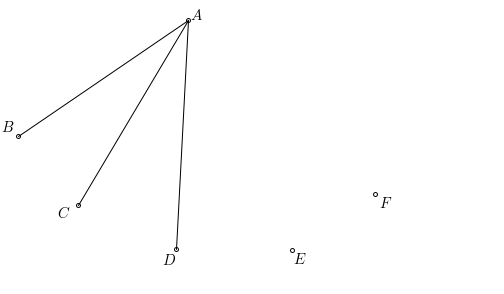
\includegraphics[scale=2.3]{r33.png}
	\end{figure}
	
	\noindent Na slici su grane jedne boje obojene u crno, dok su ostale bele (ne vide se).
	Neka su, bez umanjenja opštosti, grane čvora A koje su incidentne sa čvorovima B, C i D obojene istom bojom (crnom). Sada postoje dve mogućnosti: 
	\vspace{1em}
	\\
	$1^\circ$ Sve grane koje povezuju čvorove B, C i D su obojene belom bojom Tada čvorovi B, C, i D obrazuju kompletan graf reda 3 obojen belom bojom.
	\vspace{0.5em}
	\\
	$2^\circ$ Bar jedna od grana koje povezuju čvorove B, C i D je obojena crnom bojom. Bez umanjenja opštosti, neka je to grana koja povezuje B i C. Tada čvorovi A, B i C sačinjavaju kompletan graf reda 3 obojen crnom bojom.
	\vspace{0.5em}
	\\Dokazali smo da je $6 \rightarrow (3, 3)$, a sada još treba dokazati da ne važi $5 \rightarrow (3, 3)$. Za to je dovoljno da pronađemo kontra primer bojenja u kojem uslov nije ispunjen:
	\begin{figure}[h]
	\centering
	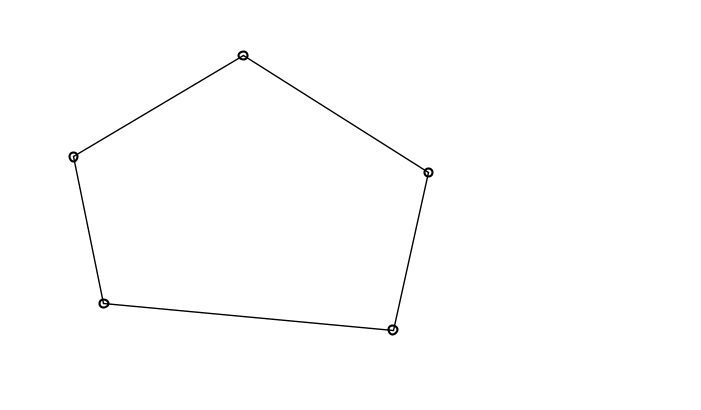
\includegraphics[scale=1.1]{r33kp.png}
	\end{figure}
	
	Dakle, $R(3,3)=6$ .	
	
	\newpage
	
	{\noindent\fontsize{12pt}{12pt}\textbf{Teorema 2.1}}
	\vspace{0.5em}	
	\\
	(1) {} {} $R(1, m) = R(m, 1) = 1$\\
	(2) {} {} $R(2, m) = R(m, 2) = m$\\
	(3) {} {} $R(l_{1}, l_{2}) = R(l_{2}, l_{1})$\\
	(4) {} {} $l \leq r \Rightarrow R(l, m) \leq R(r, m)$\\
	
	{\noindent\fontsize{12pt}{12pt}\textbf{Dokaz 2.1}}
	
	\vspace{0.5em}
	
	\noindent(1) {} {} U grafu reda 1 uvek postoji kompletan podgraf reda 1 čije su sve grane obojene istom bojom, stoga broj $m$ ne utiče na $R(1, m)$.
	\vspace{0.5em} 	\\
	\noindent(2) {} {} U grafu reda m, ili su sve grane obojene jednom bojom, ili postoji bar 1 grana koje je obojena različitom bojom od ostalih. Ako su sve grane obojene jednom bojom imamo kompletan podgraf reda $m$ čije su sve grane obojene istom bojom. Sa druge strane, ako postoji grana koja je obojena različitom bojom, čvorovi sa kojima je ta grana incidentna indukuju podgraf reda $2$ čije su sve grane obojene jednom bojom.
	\vspace{0.5em} \\
	\noindent(3) {} {} Redosled $l_{1}$ i $l_{2}$ ne utiče na $R(l_{1}, l_{2})$ jer sve za svako bojenje grana boje mogu obrnuti.
	\vspace{0.5em} \\
	\noindent(4) {} {} Pretpostavimo suprotno: $l \leq r \Rightarrow R(l, m) > R(r, m)$. Kako je $R(r, m) \rightarrow (r,m)$ i  $l \leq r$, sledi $R(r, m) \rightarrow (l, m)$, ali onda $R(l, m)$ nije Remzijev broj za $(l,m)$ jer postoji broj manji od njega koji je dovoljan za $(l, m)$. Kontradikcija.
	\vspace{1.5em}
	
	{\noindent\fontsize{12pt}{12pt}\textbf{Teorema 2.2}}
	\vspace{0.5em}	
	\\
	Za sve $m,n \geq 2$ važi
	\[R(m,n) \leq {m+n-2\choose m-1} = {m+n-2\choose n-1}\]
	\vspace{1em}
	{\noindent\fontsize{12pt}{12pt}\textbf{Dokaz 2.2}}	\vspace{-0.5em}
	\\
	\noindent Ovu teoremu dokazaćemo indukcijom.\\
	Baza indukcije:\\
	\[R(1,2) = R(2,1) = 1 \leq {1+2-2\choose 1-0}={1\choose 0}=1\]\\
	Indukcijska hipoteza:
	Neka tvrđenje važi za sve $(p,q)<(m,n)$.\\
	Indukcijski korak: po indukcijskoj hipotezi važi 
	\[R(m-1, n) \leq {m+n-3\choose m-2} \quad tj. \quad {m+n-3\choose m-2}\rightarrow (m-1, n)\] 
	\[R(m, n-1) \leq {m+n-3\choose m-1} \quad tj. \quad {m+n-3\choose m-1}\rightarrow (m, n-1)\]
	
	Sada iz Paskalove formule i Teoreme 1.? sledi 
	\[{m+n-3\choose m-2}+{m+n-3\choose m-1}={m+n-2\choose m-1}\rightarrow (m,n)\] 
	\\
	\vspace{0.7em} tj. $R(m,n) \leq {m+n-2\choose m-1}$, što je i trebalo dokazati. 
	
	{\noindent\fontsize{12pt}{12pt}\textbf{Teorema 2.3}}
	Za $m,n\geq 2$  važi sledeće:
	
	\[
   	 R(m,n)\leq 
		\begin{cases}
    		R(m-1,n)+R(m,n-1)-1,& \text{ako su R(m-1,n) i R(m,n-1) parni}\\
    	R(m-1,n)+R(m,n-1),      & \text{inače}
	\end{cases}
	\]
	
	{\noindent\fontsize{12pt}{12pt}\textbf{Dokaz 2.3}}
	Iz teoreme 1.obrad već znamo da važi
	\[R(m,n)\leq R(m-1,n)+R(m,n-1),\]
	a sada još treba dokazati da je
	\[R(m,n)\leq R(m-1,n)+R(m,n-1)-1\] 
	ako su $R(m-1,n)$ i $R(m,n-1)$ parni.
	\vspace{0.5em}
	\\
	\noindent Neka je $t=R(m-1,n)+R(m,n-1)-1$.
	Znamo da je t neparan broj. Posmatrajmo graf G sa t čvorova čije su grane obojene u dve boje: crvenu i plavu. Neka je T podgraf grafa G koji se sastoji iz plavih grana i svih čvorova grafa G. Neka je $\delta(v_i)$ stepen i-tog čvora u grafu T. Iz Prve teoreme teorije grafova znamo da je zbir stepeni svih čvorova u grafu paran broj. Kako u grafu T ima neparan broj čvorova (broj čvorova je t, isto kao i u grafu G), sledi da bar jedan čvor mora imati paran stepen. Neka to, bez umanjenja opštosti, bude čvor $v_1$ i neka je njegov stepen $d_1$. To znači da je čvor $v_1$ incidentan sa parnim brojem plavih grana. Posmatrajmo sada ostale čvorove u grafu G. Neka je M skup čvorova koji su sa čvorom $v_1$ povezani plavom granom, a N skup čvorova koji su sa $v_1$ povezani crvenom granom. Kako već znamo da je $|M| = d_1$,  sledi da je $|N| = t-1-d_1$, pa su $|M|$ i $|N|$ parni brojevi. Po Uopštenom Dirihleovom principu mora da važi jedno od sledećeg:
	\[|M|\geq R(m-1,n)-1 \quad \text{ili} \quad  |N|\geq R(m,n-1)\] 
	Međutim, kako znamo da je $|M|$ paran broj a $R(m-1,n)-1$ neparan broj, nejednakost se može pojačati na $|M|\geq R(m-1,n)$. \\
	Pretpostavimo da važi $|M|\geq R(m-1,n)$. To znači da podgraf grafa G indukovan čvorovima iz skupa $M$ sadrži crveni $\bf K_n$ graf (u tom slučaju je kraj dokaza) ili plavi $\bf K_{m-1}$ graf koji zajedno sa čvorom $v_1$ čini plavi $\bf K_{m}$ graf (kraj dokaza).\\
	Slučaj za $|N|\geq R(m,n-1)$ se dokazuje analogno.\\
	
	\begin{mdframed}
	{\noindent\fontsize{12pt}{12pt}\textbf{Definicija 2.2}}\\
	$(l_1, l_2)$-Remzi-graf je graf koji ne sadrži ni potpun podgraf sa $l_1$ čvorova ni nezavisan skup sa $l_2$ čvorova.
	
	\end{mdframed}
	
	Za svako $l_1$ i $l_2$ postoji konačan broj $(l_1, l_2)$-Remzi grafova, ali je određivanje njihovog tačnog broja vrlo teško, baš kao i određivanje samih Remzijevih brojeva. Da bi graf bio $(l_1, l_2)$-Remzi graf, on ne sme imati više of $R(l_1, l_2)-1$ čvorova.\\
	Kao što smo već videli u Primeru 2.1, graf $C_5$ je Remzi-graf za (3,3).
	
	\newpage
	

	\noindent Definicija Remzijevog broja se može uopštiti: 	
	
	\begin{mdframed}
	\vspace{0.4em}
	
	{\fontsize{12pt}{12pt}\textbf{Definicija 2.3 (Uopšteni Remzijev broj)}}
	\\
	
	\vspace{-0.8em}
	Remzijev broj $R(l_{1}, l_{2}, ... , l_{k})$ je najmanje $n \in \mathbb{N}$ \textbackslash {} $\left\lbrace 0\right\rbrace $ takvo da $n\rightarrow(l_{1}, l_{2},  ... , l_{k})$.
	\end{mdframed}
	
	{\noindent\fontsize{12pt}{12pt}\textbf{Teorema 2.4}}
	\vspace{0.4em}
	\\
	Za $c>2$ važi $R(l_1, l_2, ... , l_c) \leq R(l_1, l_2, ... , l_{c-2}, R(l_{c-1}, l_c))$
	
	\vspace{0.3em}
	
	{\noindent\fontsize{12pt}{12pt}\textbf{Dokaz 2.4}}
	\vspace{0.4em}
	
	\noindent Uočimo kompletan graf G od $R(l_1, l_2, ... , l_{c-2}, R(l_{c-1}, l_c))$ čvorova, i neka su njegove grane obojene u $c$ boja. Sada zamislimo da su $c-1$ i $c$ ista boja. Tada su grane grafa G obojene u $c-1$ boja. Tada po definiciji  $R(l_1, l_2, ... , l_{c-2}, R(l_{c-1}, l_c))$ graf G sadrži ili $K_{l_i}$ čije su grane obojene u boju $i$ za neko $1 \leq i \leq c-2$ ili sadrži $K_{R(l_{c-1}, l_c)}$ čije su grane obojene u mešanu $c-1$ i $c$ boju. Ako se radi o prvom slučaju, to je kraj dokaza. Ako se radi o drugom slučaju, to znači da imamo ili $K_{n_{c-1}}$ graf čije su grane obojene u boju $c-1$, ili $K_{n_{c}}$ graf čije su grane obojene u boju $c$, i time je dokaz završen.
	
	\newpage
	\section{Granice remzijevih brojeva}
	Kako problem određivanja tačnih vrednosti Ramsey-evih brojeva važi za ekstremno težak, umesto tačnih vrednosti, za nepoznate Ramsey-eve brojeve se određuju gornje i donje granice.
	\subsection{''Pascal-ov trougao`` za  Ramsey-eve brojeve}
	''Pascal-ov trougao`` za  Ramsey-eve brojeve se konstruiše na osnovu Teoreme 2.3 i daje gornje granice za Ramsey-eve brojeve. Koristeći već poznate Ramsey-eve brojeve, i uslov koji je dodat u Teorimi 2.3, gornje granice se mogu dodatno smanjiti.
	\vspace{0.2em}
	\noindent Ovako izgledaju prvih devet redova trougla:
	\vspace{0.5em}
	\tiny 
\[R(2,2)=2\]
\[R(2,3)=3\hspace{0.3cm}R(3,2)=3\]
\[R(2,4)=4\hspace{0.3cm}R(3,3)=6\hspace{0.3cm}R(4,2)=4\]
\[R(2,5)=5\hspace{0.3cm}R(3,4)=9\hspace{0.3cm}R(4,3)=9\hspace{0.3cm}R(5,2)=5\]
\[R(2,6)=6\hspace{0.3cm}R(3,5)=14\hspace{0.3cm}R(4,4)=18\hspace{0.3cm}R(5,3)=14\hspace{0.3cm}R(6,2)=6\]
\[R(2,7)=7\hspace{0.3cm}R(3,6)=18\hspace{0.3cm}R(4,5)=25\hspace{0.3cm}R(5,4)=25\hspace{0.3cm}R(6,3)=18\hspace{0.3cm}R(7,2)=7\]
\[R(2,8)=8\hspace{0.3cm}R(3,7)=23\hspace{0.3cm}R(4,6)\leq 43\hspace{0.3cm}R(5,5)\leq 50\hspace{0.3cm}R(6,4)\leq 43\hspace{0.3cm}R(7,3)=23\hspace{0.3cm}R(8,2)=8\]
\[R(2,9)=9\hspace{0.3cm}R(3,8)=28\hspace{0.3cm}R(4,7)\leq 66\hspace{0.3cm}R(5,6)\leq 93\hspace{0.3cm}R(6,5)\leq 93\hspace{0.3cm}R(7,4)\leq 66\hspace{0.3cm}R(8,3)=28\hspace{0.3cm}R(9,2)=9\]
\[R(2,10)=10\hspace{0.3cm}R(3,9)=36\hspace{0.3cm}R(4,8)\leq 94\hspace{0.3cm}R(5,7)\leq 159\hspace{0.3cm}R(6,6)\leq 186\hspace{0.3cm}R(7,5)\leq 159\hspace{0.3cm}R(8,4)\leq 94\hspace{0.3cm}R(9,3)=36\hspace{0.3cm}R(10,2)=10\]
\normalsize
\subsection{Donje granice za Ramsey-eve brojeve oblika R(k,k)}
{\noindent\fontsize{12pt}{12pt}\textbf{Teorema 3.1}}
Neka su dati prirodni brojevi $n$ i $k$, takvi da $n\geq k>0$. Ako je
\[\binom{n}{k}2^{1-\binom{k}{2}}<1,\]
onda važi $R(k,k)>n$.\\
{\noindent\fontsize{12pt}{12pt}\textbf{Dokaz 3.1}} todo!\\
{\noindent\fontsize{12pt}{12pt}\textbf{Teorema 3.2}} Postoji $c>0$, takvo da za sve $k\in \mathbb{N}\setminus\{0\}$ važi:
\[R(k,k)\geq c\cdot k\cdot\sqrt{2^k}\]\\
{\noindent\fontsize{12pt}{12pt}\textbf{Dokaz 3.2}} todo!
\subsection{Poznate granice}
Do sada poznate netrivijalne granice se mogu videti u sledećoj tabeli:\\
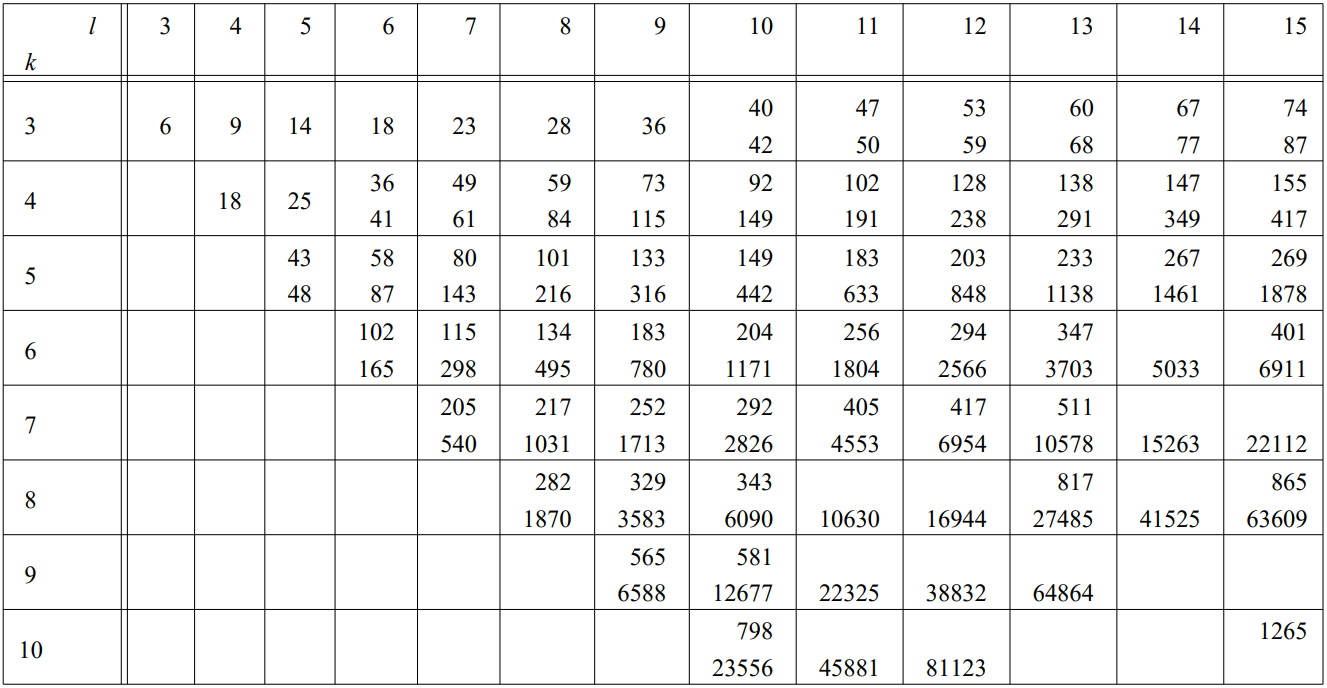
\includegraphics[width=\textwidth]{poznateGranice.png} %Uzeto sa https://www.combinatorics.org/ojs/index.php/eljc/article/view/DS1
\end{document}